\title{Weekly Progress: 7 July - 13 July 2014}
\author{}
\date{\today}

\documentclass[10pt,letterpaper]{article}

\usepackage{fullpage}	% Give me 1in margins all around
\usepackage{graphicx}	% For including pictures
\usepackage[colorlinks=true,linkcolor=blue,urlcolor=blue]{hyperref}	% For hyper links
\usepackage{parskip}	% No paragraph indention
\usepackage[small,compact]{titlesec}	% Less spacing between titles
\usepackage{listings}	% For including code
\usepackage{amsmath}	% for plain text in math mode
\usepackage{amsfonts}	% For mathy lettering
\usepackage{algpseudocode}	% For pseudocode typesetting
\usepackage{subfig}		% For subfigures
\usepackage[margin=1in]{geometry}

\begin{document}

\maketitle

All of the source code for this work can be found on GitHub at:

\url{http://github.com/cbuntain/ChangePointDetection}

\section{Achievements}

\begin{itemize}
\item \textbf{Procured Bitcoin market value data across four currencies} -- We acquired the MtGox Bitcoin exchange data from Quandl.com (link here: \url{http://www.quandl.com/markets/bitcoin-data}). This data set covers 3 October 2011 to 25 February 2014 (when MtGox was shut down).
\item \textbf{Developed a test suite for the LRT and Cusum algorithms} -- This suite supports testing across various dimensions of data ($k \in 2\cdot \mathbb{N}[1, 15]$), a range of change points ($[0, 10]$), randomly generated $\Phi$ matrices, and randomly generated data means. Each run of the test suite can perform an arbitrary number of runs across an arbitrary time series size, which are currently set to 500 and 10,000 respectively.
\begin{itemize}
\item $\mathbf{\Phi}$ \textbf{Generation} -- Generating satisfactory $\Phi$ matrices is a non-trivial task as randomly generated matrices tend to violate constraints needed for VAR processing. To synthesize constraint-satisfying matrices, we performed the following:

\begin{enumerate}
\item Generate a sparse $k \times k$ candidate matrix $\Phi_c$ with density=0.25. Ssparse matrices were used to avoid issues with generating a full $k \times k$ set of satisfactory values, which is unlikely for large $k$ and results in long loops trying to generate good matrices.
\item Construct a new matrix $\Phi_c = \Phi_c + \Phi_c^T + zI$ where $z$ is some random integer in $[2, 9]$. This formula was used to ensure non-singular $\Phi$.
\item Calculate the eigenvalues $\lambda$ for the candidate $\Phi_c$ and use them to determine whether the zeros of the equation of the determinant $|\Phi_c(x)| = |I - \Phi_{c1}x_{t1} ...|$ are on or outside the unit disk. To ensure this, we need to ensure all $\lambda^{-1} > 1$. If not, we try to scale down the $\Phi_c$ matrix by multiple by $(\text{max}(\lambda)+1)^{-1}$. If this scaling still does not provide satisfactory $\Phi_c$, we restart the process with a new candidate.
\end{enumerate}

\item \textbf{Result logging} -- Running logs of the suite's execution are saved to a log file, and results such as identified versus actual change points and computed $W$ matrices are stored in a JSON file for review.
\item \textbf{Accuracy and scoring} -- The number of true positives, false positives, and false negatives are also calculated for each run of each algorithm. A true positive is defined as a change point detected within $\pm 20$ time steps of the actual change point. False positives are identified change points outside this range, and false negatives are change points missed by the algorithms. Once the test suite has finished its runs, it then calculates the accuracy and F1 score for each algorithm.
\item \textbf{Compared LRT and Cusum across dimensions} -- With the test suite, we were able to compare the relative performance of LRT and Cusum as $k$ increases (see Figure \ref{fig:lrtVcusum}). Increases in $k$ reduce accuracy in both algorithms, but Cusum is much more sensitive to this change.
\item \textbf{Identified a problem for high-dimensional data} -- According to Galeano and Pe\~{n}a's paper, one should use some interval $2d$ as the minimum set size to compare and when determining whether two potential change points are the same. This $d$ is quadratic with respect to $k$, so when $k$ is large, the minimum amount of data needed to identify a change point is very large. This issue makes sentiment analysis for relatively high-dimensional data like Twitter problematic.
\end{itemize}

\item \textbf{Wrote cleaner pseudocode for the Cusum algorithm} -- The procedure as detailed in Galeano and Pe\~{n}a's paper is not very clear on several points. We drafted a cleaner description of the implementation for future reference. 
\item \textbf{Implemented Desobry's Kernel Change Detection algorithm} -- Leveraged Python's Scikit package and its OneClassSVM implementation to construct dissimilarity indices for points in a given time series. This algorithm uses a sliding window of size $2m$ to calculate this index for a given $t$ and compares it against a user-provided threshold $\eta$ (generally, $\eta \in [0, 1]$).

\begin{itemize}
\item \textbf{Preliminary experimentation} -- This algorithm seems to work well for structural changes such as mean shifts but does not seem well-suited to discriminating two regimes between which only the covariance changes (Figure \ref{fig:kcdDiff}). We are currently exploring feature extractors to provide better information in this regard.
\end{itemize}

\item \textbf{Ran Bitcoin data through LRT, Cusum, and KCD} -- We searched for change points in the Bitcoin data using all three algorithms currently implemented. Results are shown in Table \ref{tab:bitcoin}.

\end{itemize}

\begin{figure}[htbp]
\begin{center}
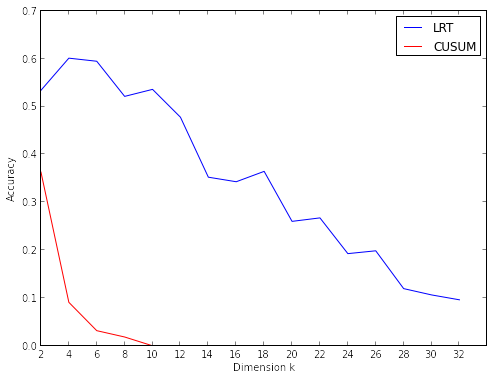
\includegraphics[width=0.66\textwidth]{LrtVCusum.png}
\caption{Accuracy of LRT versus Cusum}
\label{fig:lrtVcusum}
\end{center}
\end{figure}

\begin{figure}[htbp]
    \centering
    \subfloat[Covariance Shift]{{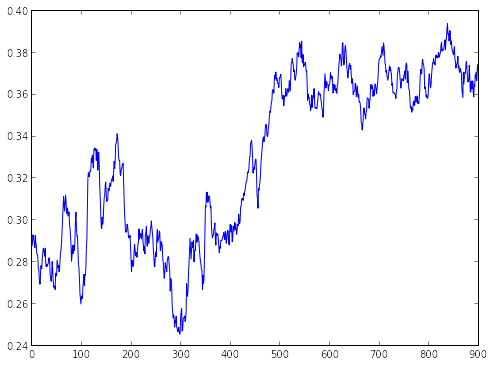
\includegraphics[width=0.66\textwidth]{kcdCovChange} }}%
    \qquad
    \subfloat[Mean Shift]{{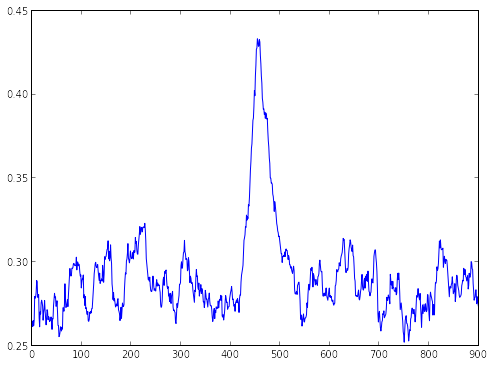
\includegraphics[width=0.66\textwidth]{kcdMeanChange} }}%
    \caption{KCD Indices}%
    \label{fig:kcdDiff}%
\end{figure}

\clearpage 

\begin{table}[htbp]
\caption{Detected Change Points}
\begin{center}
\begin{tabular}{|c|c|c|}
\hline
\textbf{LRT} & \textbf{Cusum} & \textbf{KCD} \\ \hline
11/13/11 &  & \\ \hline
12/29/11 &  &  \\ \hline
1/20/12 &  &  \\ \hline
3/27/12 &  &  \\ \hline
5/13/12 &  &  \\ \hline
6/7/12 &  &  \\ \hline
7/4/12 & 7/14/12 & 7/7/12  \\ \hline
7/31/12 &  & 8/2/12 \\ \hline
9/6/12 & 8/26/12 &  \\ \hline
12/11/12 &  & 12/17/12 \\ \hline
1/19/13 & 1/19/13 &  \\ \hline
2/28/13 &  &  \\ \hline
3/26/13 & 3/9/13 & 3/26/12 \\ \hline
5/3/13 & 5/3/13 &  \\ \hline
6/6/13 &  & 7/25/13 \\ \hline
10/15/13 &  &  \\ \hline
11/5/13 & 11/9/13 &  \\ \hline
\end{tabular}
\end{center}
\label{tab:bitcoin}
\end{table}

%\clearpage

\section{Plans for the Upcoming Week}

\begin{itemize}
\item \textbf{Evaluate implementations on other model types} -- Since our current implementations of LRT and CUSUM statistics rely on a library that can only perform MLEs for VAR-based series, we need to figure out how well (if at all) this works for VARMA or VARIMA and models of different $(p,d,q)$ orders.
\item \textbf{Continue implementing online algorithms} -- We need to finish implementation of the fourth algorithm.
\item \textbf{Dive deeper into the bridge and Bitcoin data sets} -- While we have some data on detected change points, we need to figure out whether those change points actually correspond to real-world events.
\end{itemize}

%\bibliographystyle{abbrv}
%\bibliography{sources}

\end{document}